\section{Pappus's harmonic theorem}

\subsection{Constructive statement}

Let $A,B,Y$ be distinct collinear affine points, let $Z$ be off their line, and let $D$ be a point of $AZ$ distinct from $A,Z$.  Define
\[
C=DY\cap ZB,
\qquad X=AC\cap DB,
\qquad W=ZX\cap AB,
\]
with the displayed intersections nondegenerate.  Then the four points $A,B,W,Y$ form a harmonic range:
\[
\crat{A}{B}{W}{Y}=-1.
\]
In the MathWorld order $A-W-B-Y$, this says that the three directed lengths $AW,AB,AY$ are in harmonic progression.

\begin{center}
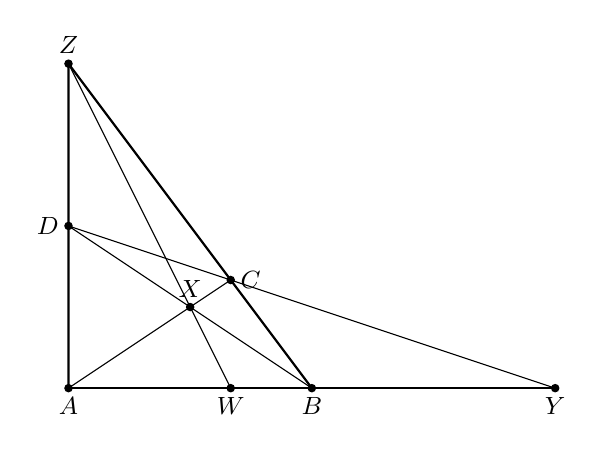
\begin{tikzpicture}[scale=1.03, every node/.style={font=\small}]
  \coordinate (A) at (0,0);
  \coordinate (W) at (2,0);
  \coordinate (B) at (3,0);
  \coordinate (Y) at (6,0);
  \coordinate (Z) at (0,4);
  \coordinate (D) at (0,2);
  \coordinate (C) at (2,1.3333);
  \coordinate (X) at (1.5,1);
  \draw[thick] (A)--(Y);
  \draw[thick] (A)--(Z)--(B);
  \draw (D)--(Y);
  \draw (A)--(C);
  \draw (D)--(B);
  \draw (Z)--(W);
  \foreach \P/\pos in {A/below,W/below,B/below,Y/below,Z/above,D/left,C/right,X/above}
    {\fill (\P) circle (1.5pt) node[\pos] {$\P$};}
\end{tikzpicture}
\end{center}

\subsection{Coordinate proof}

Apply the constructive affine normalization of the previous section:
\[
A=(0,0,1),\quad B=(1,0,1),\quad Z=(0,1,1).
\]
Because $Y\in AB$ and $D\in AZ$, write
\[
Y=(t,0,1),\qquad D=(0,d,1),
\]
where $d\ne0,1$.  Repeated use of join and meet gives representatives
\begin{align*}
C&=(D\join Y)\meet(Z\join B)\\
 &\sim\bigl(t(d-1),\;-d(t-1),\;d-t\bigr),\\[0.3em]
X&=(A\join C)\meet(D\join B)\\
 &\sim\bigl(-dt(d-1),\;d^2(t-1),\;-d(dt-2t+1)\bigr),\\[0.3em]
W&=(Z\join X)\meet(A\join B)\\
 &\sim -d(d-1)\bigl(t,0,2t-1\bigr).
\end{align*}
Since $d(d-1)\ne0$, we may take
\[
W\sim(t,0,2t-1).
\]
In particular, $W$ is independent of the auxiliary choice of $D$.

Identify the projective baseline $AB$ with $\mathbf P^1$ by retaining the first and third homogeneous coordinates.  Thus
\[
A=(0:1),\quad B=(1:1),\quad Y=(t:1),\quad W=(t:2t-1).
\]
For two line points $P=(p_0:p_1)$ and $Q=(q_0:q_1)$ write
$[P,Q]=p_0q_1-p_1q_0$.  The division-free harmonic condition is
\[
[A,W][B,Y]+[A,Y][B,W]=0.
\]
Here
\[
[A,W]=-t,\quad [B,Y]=1-t,\quad [A,Y]=-t,\quad [B,W]=t-1,
\]
and the sum is zero.  Therefore $\crat{A}{B}{W}{Y}=-1$.

If $2t-1\ne0$, then $W$ is finite with affine coordinate
\[
w=\frac{t}{2t-1}.
\]
Taking $AB=1$ and $AY=t$ gives
\[
\frac1{AW}+\frac1{AY}=\frac{2t-1}{t}+\frac1t=2=\frac2{AB},
\]
which is exactly the harmonic-progression formulation appearing in elementary accounts.

\subsection{Constructive audit}

The proof consists of fixed polynomial expressions and one cancellation by $d(d-1)\ne0$.  The harmonic conclusion is stated without division and therefore also covers the case $2t-1=0$, where $W$ is the point at infinity of $AB$.  No order or betweenness argument is used; the picture's order is only needed to reinterpret the directed relation as a positive-length harmonic progression.
